% !TeX encoding = UTF-8
% !TeX spellcheck = en_US
% !BIB TS-program = biber
% basic packages and document settings
\documentclass[a4paper,12pt]{article}
\usepackage[english]{babel}
\usepackage[utf8]{inputenc}
\usepackage[T1]{fontenc}
\usepackage[a4paper]{geometry}
\geometry{top = 30mm, bottom = 25mm, left = 25mm, right = 25mm}
\usepackage{setspace}
\onehalfspacing
\raggedbottom
\pdfcompresslevel9

% mathmode-related packages
\usepackage{mathtools}
\usepackage{physics}
\usepackage{amsmath}
\usepackage{amsthm}
\usepackage{amsbsy}
\usepackage{mathrsfs}
\usepackage{amssymb}
\usepackage{amstext}
\usepackage{amsfonts}
\usepackage{tikz}
\usepackage{siunitx}
%\usepackage{IEEEtrantools}

% misc
\usepackage{esdiff}
\usepackage{multirow}
\usepackage{blindtext}
\usepackage{todonotes}
\usepackage{abstract}
\usepackage{appendix}
\usepackage[bottom]{footmisc}
\usepackage{listings}
\usepackage{dashrule}

% graphics and floats
\usepackage{graphicx}
\graphicspath{{../Figures/}}
\usepackage{tikz}
\usepackage{float}
\usepackage{wrapfig}
%\usepackage{subfloat}
\usepackage{subcaption}
%\usepackage{caption}
\usepackage[rightcaption]{sidecap}
\usepackage{tabularx}
\usepackage{adjustbox}
%\usepackage{svg}
\usepackage{epstopdf}
\usepackage{grffile}	% handle file names with dots, spaces etc.
%\usepackage{flafter}
\usepackage{rotating}
%\usepackage{floatrow}
%\floatsetup[figure]{capposition=beside,capbesideposition={top,right}}

%\usepackage{epstopdf}
%\epstopdfDeclareGraphicsRule{.pdf}{png}{.png}{convert #1 \OutputFile}
%\AppendGraphicsExtensions{.pdf}

% packages requiring setup arguments

\usepackage{xcolor}
%\definecolor{rwth-dark}{HTML}{176daf}
\definecolor{rwth-dark}{RGB}{0,84,159}
%\definecolor{rwth-light}{HTML}{8abae3}
\definecolor{rwth-light}{RGB}{142,186,229}

%/**
%* Generated by Gpick 0.2.5
%* RWTH Dark: #176daf, rgb(23, 109, 175), hsl(32, 43%, 69%)
%* RWTH Light: #8abae3, rgb(138, 186, 227), hsl(195, 73%, 89%)
%*/

\usepackage{hyperref}
\hypersetup{hidelinks=true,colorlinks=true,allcolors=rwth-dark}
\usepackage[nameinlink,capitalise]{cleveref}
%\usepackage[hyphens]{url}
%\urlstyle{sf}
%\usepackage{breakurl}


% header & footer settings
\usepackage{fancyhdr}
\pagestyle{fancy}
%\renewcommand{\chaptermark}[1]{\markboth{#1}{}} % with this we ensure that the chapter and section headings are in lowercase.
\renewcommand{\sectionmark}[1]{\markright{\thesection\ #1}}
\fancyhf{} % delete current header and footer

%\fancyhead[LE,RO]{\large\thepage}
\fancyhead[L]{\large\rightmark}
\fancyhead[R]{\large\thepage}

\renewcommand{\headrulewidth}{0.3pt}
\renewcommand{\footrulewidth}{0pt}
%\addtolength{\headheight}{0.5pt} % space for the rule

\fancyfoot[C]{\thepage}

\fancypagestyle{plain}
{
	\fancyhead{} % get rid of headers on plain pages
	\renewcommand{\headrulewidth}{0pt} % and the line
}

% ========== command definitions =================================
\newcommand{\Thickline}{\rule{\linewidth}{0.4mm}}
\newcommand{\Thinline}{\rule{\linewidth}{0.1mm}}

\newcommand{\id}{\, \mathrm{d}}

\definecolor{codegray}{gray}{0.9}
\newcommand{\code}[1]{\colorbox{codegray}{\texttt{#1}}}

\newcommand{\skippage}{\clearpage{\thispagestyle{empty}\cleardoublepage}}

\def\@esphack{%
	\relax
	\ifhmode
	\spacefactor\@savsf
	\ifdim\@savsk>\z@
	\ignorespaces
	\fi
	\fi}

\title{\LARGE title}
\date{}


\begin{document}
	
\begin{titlepage}
	\thispagestyle{empty}
	\newgeometry{top=20mm, left=20mm, right=20mm, bottom=20mm}
	
%	\begin{minipage}{0.35\textwidth}
%		\begin{flushleft}
%
%
%		\end{flushleft}
%	\end{minipage}
%	\hfill
%	\begin{minipage}{0.65\textwidth}
%		\begin{flushright}
%
%		\end{flushright}
%	\end{minipage}
	
%	\vspace*{\fill}
	\hspace{0pt}
	\vspace{2cm}
	\begin{center}
%		\Thickline
%		\vskip -0.5cm
%		\Thinline
		\hdashrule{\linewidth}{1pt}{}
		\vskip -0.5cm
		\hdashrule{\linewidth}{0.5pt}{}
		
		\vspace{0.5cm}
		\Huge{ \textbf{ F3 \\}}
		\LARGE{ \textbf{Rastertunnelmikroskopie} } 
		
		\hdashrule{\linewidth}{0.5pt}{}
		\vskip -0.95cm
		\hdashrule{\linewidth}{1pt}{}
%		\Thinline
%		\vskip -0.9cm
%		\Thickline 
		
		\vspace{3cm}
		\Large{\textbf{ Gruppe 14 \\}}
		\Large{Heithem Assili, ****** \\ Alexandre Drouet, 358681 \\ Olexiy Fedorets, 356615 \\}
		\vspace{1cm}
		\Large{\textsl{ Versuchstag: 12.03.2019 \\ Protokollabgabe: 27.03.2019}}

		

		
	\end{center}
	\vfill
%	\vspace*{\fill}
	
\end{titlepage}
	
	
	
\skippage
\pagenumbering{roman}
\thispagestyle{plain}

\tableofcontents
%	\newpage
\newpage
\listoffigures

%\begingroup
%\let\cleardoublepage\relax
%\let\clearpage\relax
\listoftables
%\endgroup
%\listoftables

\skippage

\pagenumbering{arabic}
\setcounter{page}{1}
\restoregeometry
\thispagestyle{fancy}


\section{Einleitung}


\section{Aufbau}


\section{Analyse}
\subsection{Gold}

\subsection{Hochorientierter pyrolytischer Graphit}

\begin{figure}[H]
\centering
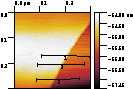
\includegraphics[width=\textwidth]{../Gwyddion/HOPG/300nm.pdf}
\caption{300nm}
\label{300nm}
\end{figure}	

\begin{figure}[H]
\centering
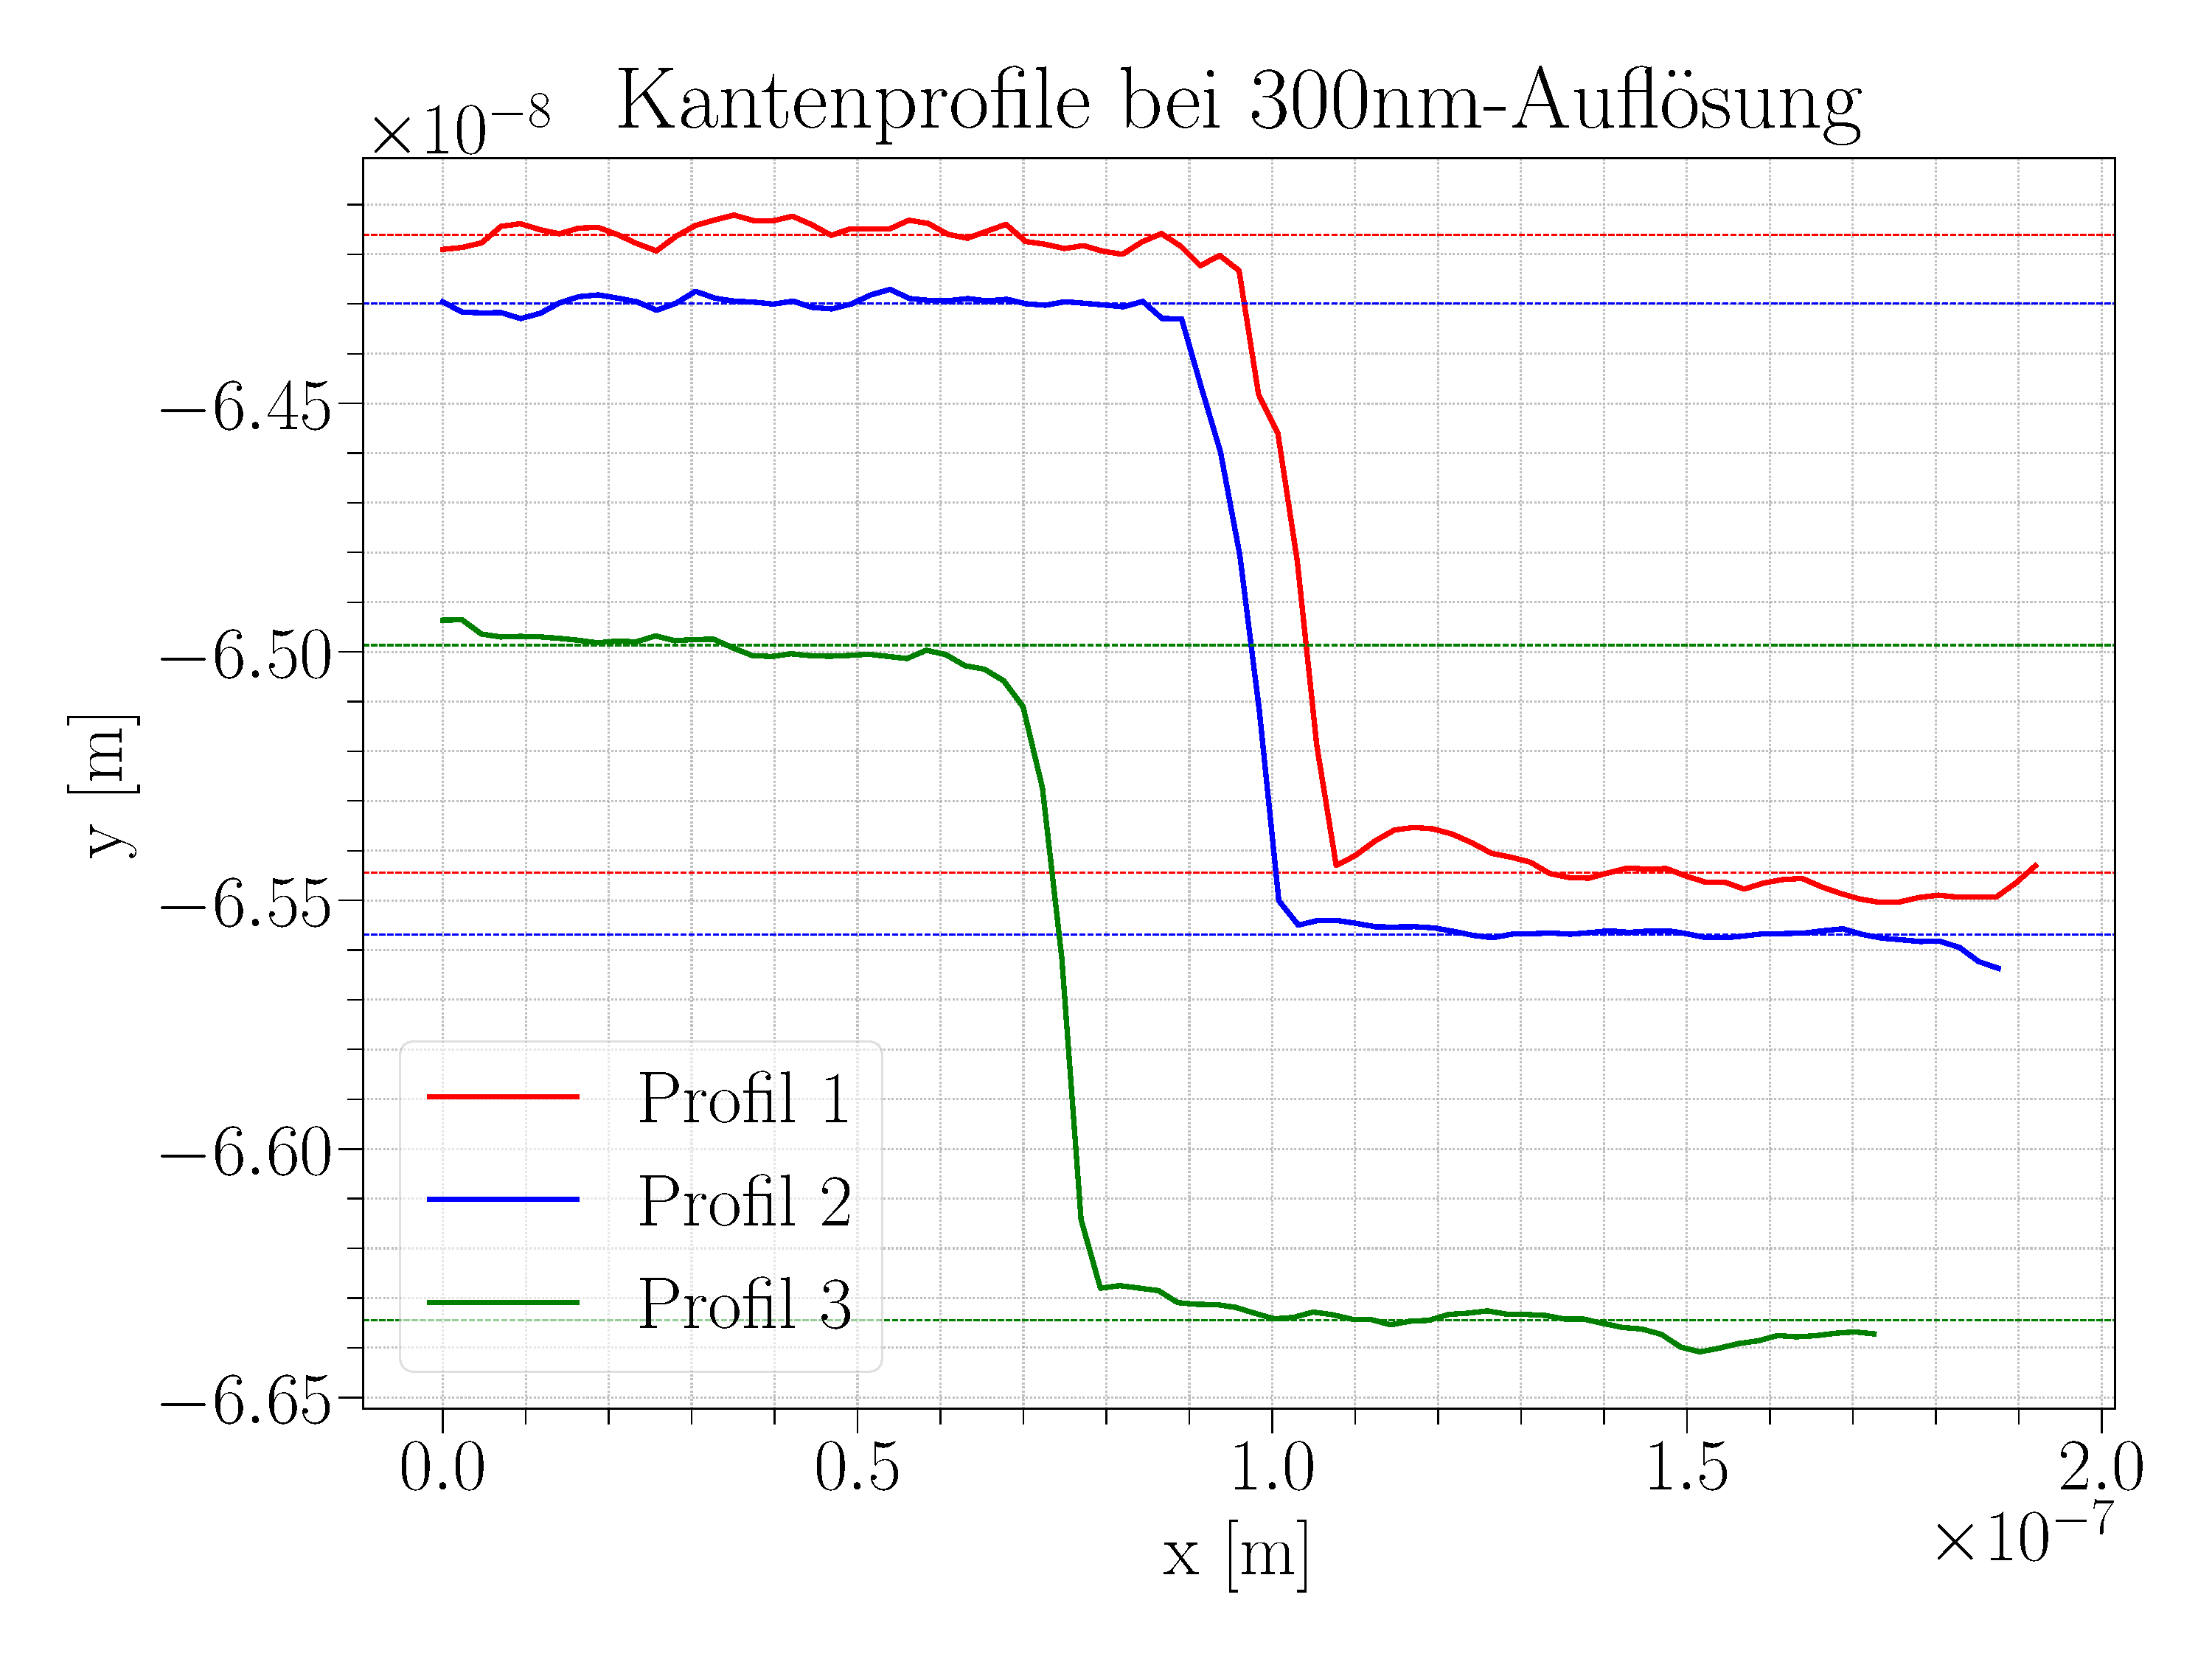
\includegraphics[width=\textwidth]{../Figures/300nm_profiles.pdf}
\caption{300nmProfiles}
\label{300nmProfiles}
\end{figure}	

\begin{figure}[H]
\centering
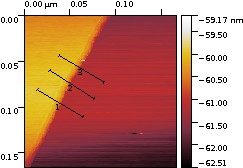
\includegraphics[width=\textwidth]{../Gwyddion/HOPG/166nm.pdf}
\caption{166nm}
\label{166nm}
\end{figure}

\begin{figure}[H]
\centering
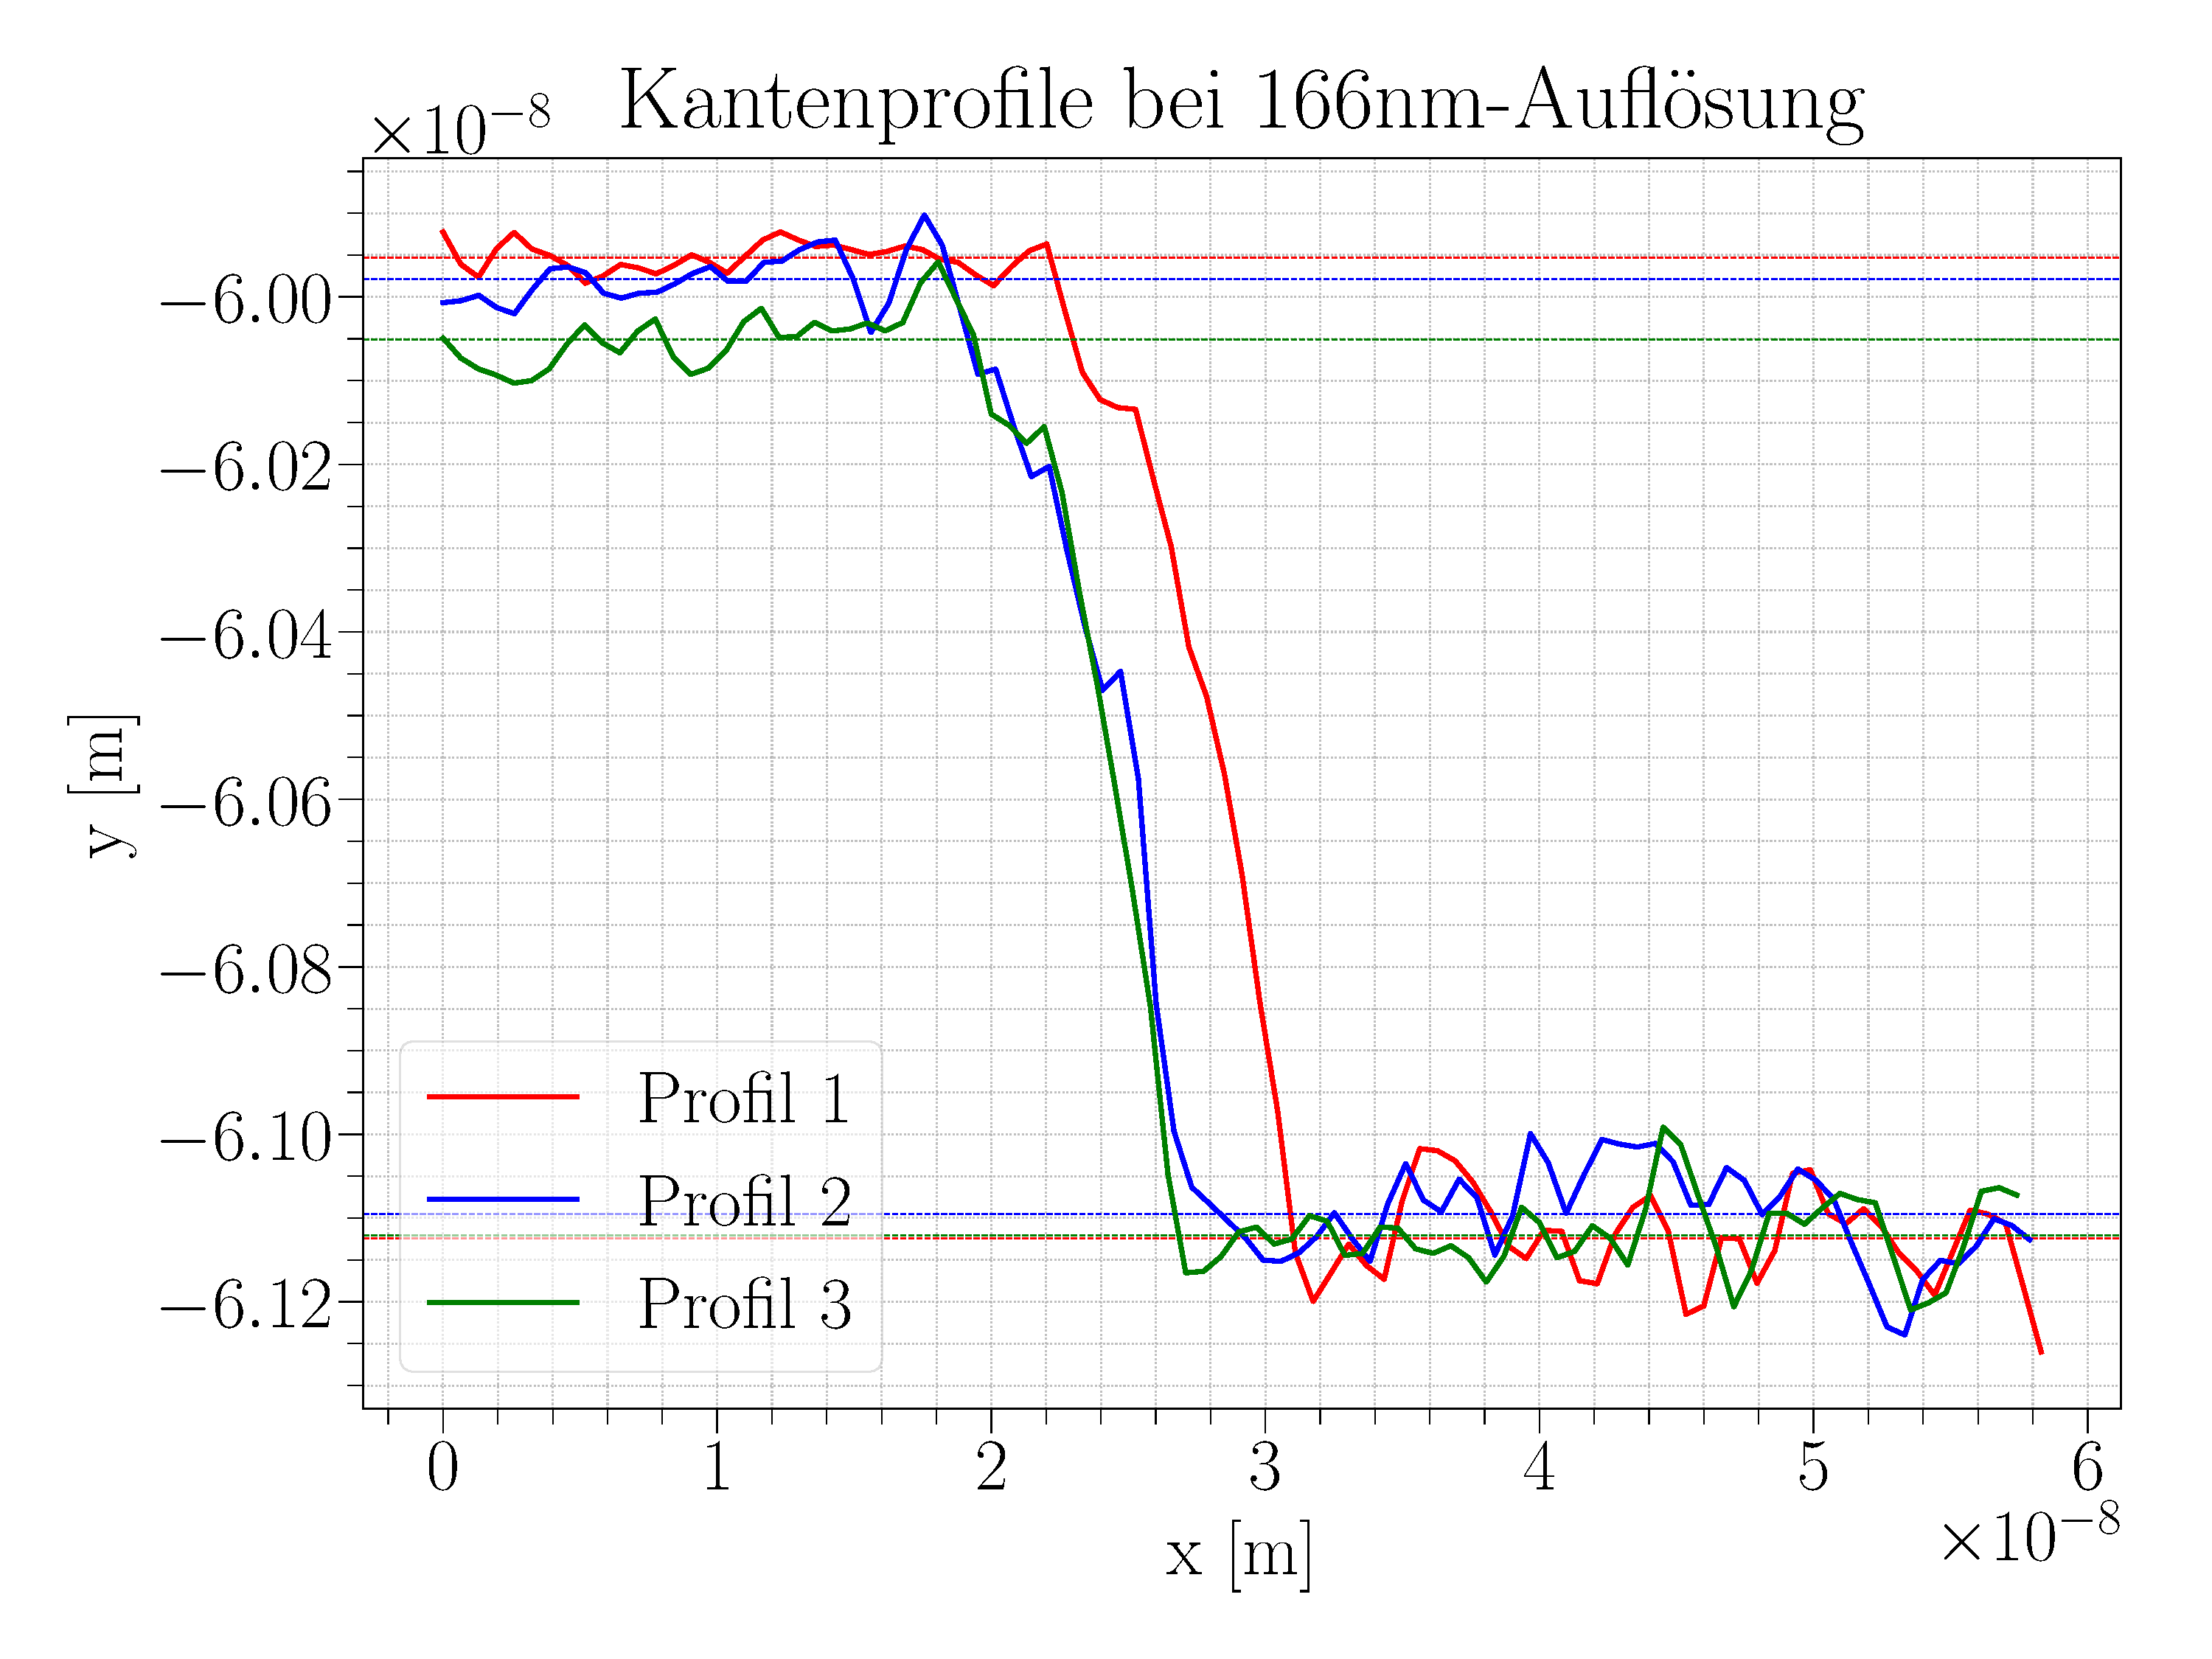
\includegraphics[width=\textwidth]{../Figures/166nm_profiles.pdf}
\caption{166nmProfiles}
\label{166nmProfiles}
\end{figure}

\begin{figure}[H]
\centering
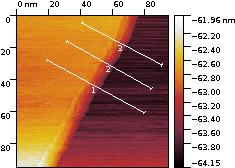
\includegraphics[width=\textwidth]{../Gwyddion/HOPG/95nm.pdf}
\caption{95nm}
\label{95nm}
\end{figure}

\begin{figure}[H]
\centering
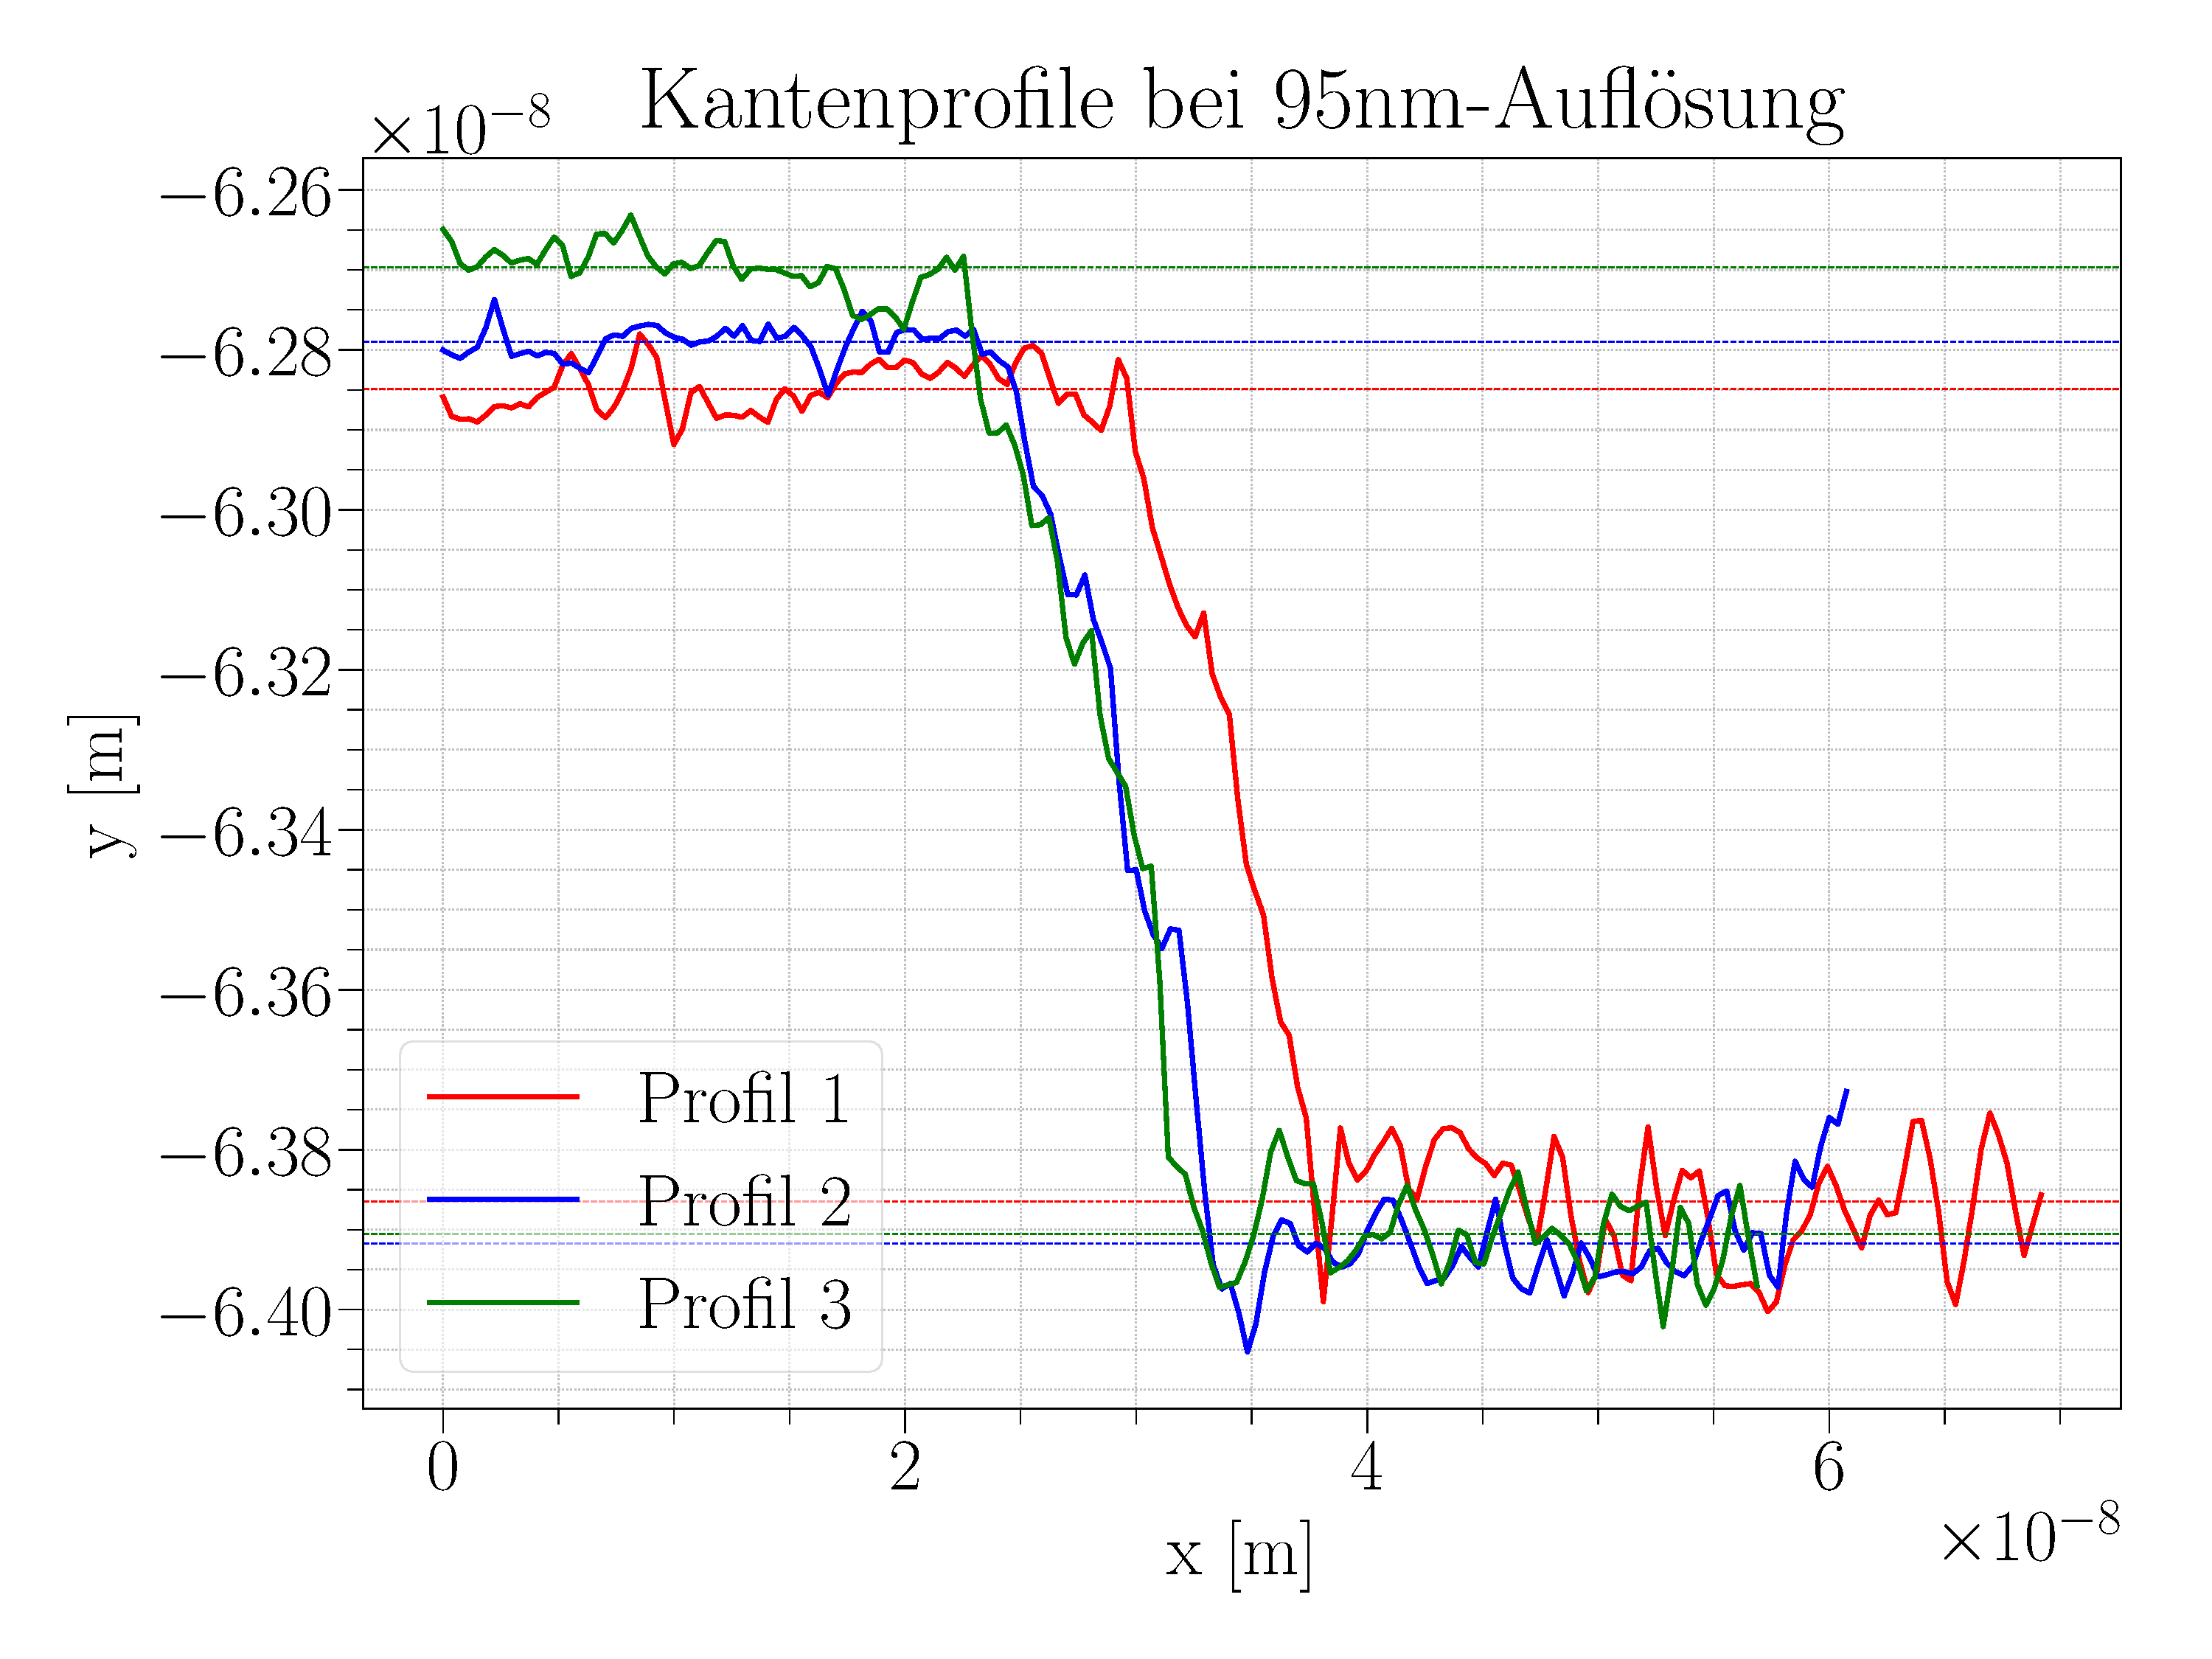
\includegraphics[width=\textwidth]{../Figures/95nm_profiles.pdf}
\caption{95nmProfiles}
\label{95nmProfiles}
\end{figure}

\begin{table}[H]
	\renewcommand{\arraystretch}{1.5}
	\centering
	\begin{tabular}{|c|c|c|c|}
		\hline
		 & individuelle Höhen ($\pm$ stat) & gewichtetes Mittel & Abweichung von der Erwartung \\
		\hline
		$K_\alpha$ & \SI{6.403}{keV} & $(6.442 \pm 0.003 \pm 0.037)$keV & $1,051\sigma$ \\
		\cline{1-4}
		 ? & ? & $(17.368 \pm 0.006 \pm 0.053)$keV & ? \\
		\hline
	\end{tabular}
	\caption{Ergebnisse der Analyse von Edelstahl.}
	\label{tab:heights}
\end{table}

\begin{figure}[H]
\centering
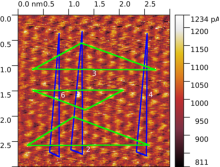
\includegraphics[width=\textwidth]{../Gwyddion/HOPG/3nm_gimped.pdf}
\caption{3nm}
\label{3nm}
\end{figure}

\begin{figure}[H]
\centering
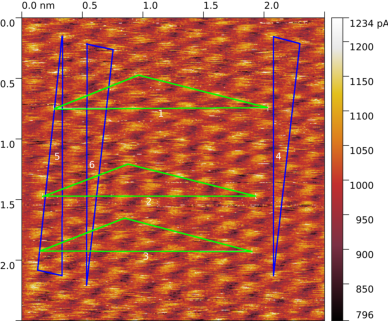
\includegraphics[width=\textwidth]{../Gwyddion/HOPG/2,5nm_gimped.pdf}
\caption{2,5nm}
\label{2,5nm}
\end{figure}

\begin{figure}[H]
\centering
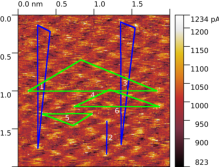
\includegraphics[width=\textwidth]{../Gwyddion/HOPG/2nm_gimped.pdf}
\caption{2nm}
\label{2nm}
\end{figure}
	
\end{document}
